{
\setlength{\parindent}{2em}
\chapter{Flight Software Checkpointing}\label{cha:das-impl}
At its core, offering a suitable environment for the simulation of the flight software was the main purpose of the BBPSim simulator. Since \gls{SNC} wanted to reproduce the in-flight behavior of the communication sub-system as faithfully as possible, the software-in-the-loop test framework was designed according to the principle of encapsulation: exclude all internal changes to the simulated software and instead build around what is already there. Having said that, inevitably, there were exceptions made for some parts of the flight software algorithms, where code had to be altered to make it compatible to run on a Linux machine. For the most part, however, as shown in \autoref{fig:bbpsim-layers}, BBPSim succeeded in integrating \gls{DAS} as an "untouchable" nucleus and interfacing only indirectly with it.

The fact that DAS was supposed to stay completely permeable to modification forced the implementation of the save \& restore feature to treat it as a black box. This point of view brought several challenges, which were not present when modifying the BBPSim code to support checkpointing. 

In this section, the constraints that influenced the development of a checkpointing technique within the flight software are first of all described. It should be noted that most of the solutions to the problems were based on technical details that, in the end, had a meaningful impact. Subsequently, \gls{DAS} is briefly analyzed to clearly define which of its components' checkpointing are considered a necessary condition for a stable restore. Then, the approach taken to indirectly access, save and restore them is explained in details.

\section{Design Constraints}
It goes without saying that user and customer requirements played a big role in how the design went forward. In particular, to make the \gls{FSW} checkpointable, it was important to bear in mind DCMS-BBP-121 (64-bit application), U02 (no alteration to FSW) and U01 (no instability). However, some other technicalities had a big importance too. They are further detailed in this chapter.

Also, since the delivery method of BBPSim was through a Linux dynamic library, it was realized that most of the container-based solutions presented in \autoref{cha:state-of-the-art} could not apply to BBPSim. A shared object does not possess the same control as an application over many things, like memory layout. This was a problem, and a better explanation of the issue is given in the coming sections.

Finally, because the build process of the dynamic library happened inside a Linux machine, the tools used to execute the checkpointing had to be standard Linux programs installed on any distribution. This constraint came from the fact that developers on the Dream Chaser team used a Linux virtual machine to run a simulation. Hence, adding in the dependency on another program would imply changing all of the Linux VMs images on the team. This was of not desirable.

\section{Definition of Sufficient Condition for Restoration}\label{sec:conditions}
Saving and restoring an application was the main subject of \autoref{cha:state-of-the-art}. In every existing solution that was presented, the checkpointer programs did not have any control over the building process of the checkpointee. This made them approach the checkpointing problem from various angles, depending on the level at which the program was supposed to interact with the checkpointed application. 

In parallel, they each introduced a different sufficient condition, in terms of what to save, to be able to restore back the checkpointee. For example, it was considered essential for CRIU to save the totality of active memory pages inside the application's \gls{VMA} range, something pointless using the C\textsuperscript{3} environment.

Since the checkpointing feature of BBPSim was done with a different set of constraints, the set of necessary conditions for a stable restore had to once again be revisited. In this section, an assessment of the required components to checkpoint in the flight software is done. 

\subsection*{Definition of FSW Program State}
The description of requirement DCMS-BBP-122 on page \pageref{tab:customer-reqs} mentioned that "the current state of the [BBPSim] model" had to be saveable between steps. Undoubtedly, the word "model" is a very abstract term, and it could be interpreted in many ways. It was important to first define what qualified as a "model" in the more concrete context of DAS.

To better picture this, a parallel can be drawn with how C code is structured once compiled. When the \gls{GCC} compiles a valid C source file on Linux, an object file with extension \texttt{.o} is produced. Internally, this file is laid out in the Unix-wide standard \gls{ELF}. This very flexible format is divided into multiple segments that each have their own function in defining the program at low-level.

In this context, there are four relevant memory segments inside an object file:
\begin{wrapfigure}{r}{0.45\textwidth}
	\centering 
	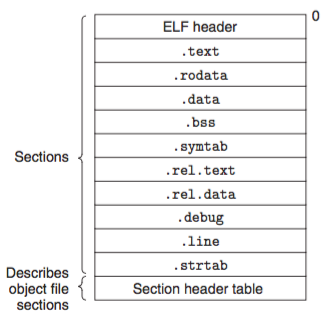
\includegraphics[width=.9\linewidth,keepaspectratio]{art/reloc-obj.png}
	\caption{Sections in an object file with ELF format.\cite{online:zhang}}
	\label{fig:sections-obj}
	\vspace{-24pt}
\end{wrapfigure}
\begin{enumerate}
	\item \textbf{\texttt{.bss}}. Contains the statically-allocated variables that were either uninitialized or initialized to zero.
	\item \textbf{\texttt{.data}}. Contains the statically-allocated variables that were initialized to zero.
	\item \textbf{\texttt{.text}}. Contains the binary instructions. Basically, the executable code.
	\item \textbf{\texttt{.rodata}}. Contains the read-only data (constants).
\end{enumerate}
\autoref{code:c-to-segments} shows how the translation is done using real C code.

In this thesis, it is argued that the state, or "model" of the flight software could be defined by two main components: the memory segments of statically-allocated variables, and the program counters. In the context of an object file, it was possible to redefine the state of a multithreaded DAS as being:
\begin{shadedquotation}
The full contents of the \texttt{.bss} and \texttt{.data} segments for all object files, the register set of each threads and the stack of each threads. 
\end{shadedquotation}

As for the \texttt{.rodata} and other segments, since they contain values that do not change from one simulation to the other, they were deemed unnecessary to include in this definition. Since they were identical at every simulation run, they were not included in the definition of the FSW state.

\subsection*{Condition 1 - Memory Segments}
The first necessary condition to be able to restore back to a previous "model" of DAS was to save the read-writeable, \textit{statically-allocated} regions in memory that concerned the flight software. It should be understood that a program's statically-allocated variables are variables that exist for the entire duration of the program. This term should not be confused with the \mintinline{c}|static| keyword of the C language, which limits the scope of a symbol in a compilation unit.

One can make an informal proof by contradiction of that statement by looking again at the sample code in \autoref{code:c-to-segments}. Let's suppose that, to restore DAS to a consistent global state, the restoration of the statically-allocated memory segments is not necessary. As a user, any changes done to variables (declared on lines \ref{lc-beg-statics} to \ref{lc-beg-statics}) during a simulation will be lost, and therefore, the global state of the application would not be consistent with the one on the previous run. Variables on the second run would not read the same as they would have at the end of the first one. The inclusion of these segments is thus a necessary condition.

\subsection*{Condition 2 - Register Sets}
A second necessary condition for a consistent DAS global state restore was to save the register set of every thread attached to the DAS program. In this set is located the \gls{PC}, depicted in \autoref{fig:x86-regs}. It is the CPU register in charge of keeping track of which instructions are to be executed. Since CPU instructions are encoded in binary and reside in the same \gls{VMA} as the variables, they are also addressable. In that sense, the program counter register holds the address of the current instruction being executed by the processor. One can think of the PC as being "where" the thread is in its execution of the program.

In addition, it was also important to save the other general-purpose registers, which contained the context of the CPU at that particular moment. Not putting the correct value in the registers would produce a domino effect resulting in a segmentation fault at best, or undefined behavior at worst.

\subsection*{Condition 3 - Thread Execution Stacks}
Finally, saving the thread execution stacks was considered the last necessary condition to make the checkpointing feature work in the context of the flight software. An execution stack contains a lot of very important information about the thread. For instance, the function-local (scoped) variables are located in this stack. For reasons similar to the first condition, it was also important to save them.

On top of that, even though the program counter represents the position of the execution of a thread at a certain time $t$, the stack also contains its \textit{backtrace}, information about the "path" taken by the thread to get there. Precisely, the backtrace (or stack trace) is defined as the series of functions that were called consecutively until $t$. The stack-related concepts are treated thoroughly in \autoref{sec:das-exec-restore}.

\subsection*{Building the Sufficient Condition}
When the three conditions listed above were grouped together, it was defined that this formed a sufficient condition for a consistent DAS global state restore. More formally, this thesis argues that:
\begin{itemize}
	\item with $F$ being a C function in DAS;
	\item with $G_s$ being the global state of DAS in memory in a first BBPSim run;
	\item with $S_r$ being a previously saved state being restored in a second BBPSim run;
\end{itemize}
then
\begin{equation} \label{eq:sr_equiv}
	\forall F: F(G_s)\equiv F(S_r)
\end{equation}
when $F$ is void of non-deterministic processes. All DAS functions satisfied to this criteria, because they were strictly exempt of dynamic memory allocation, random numbers, and scheduling non-determinism (since the order of execution for threads was set at compile-time).

It should be noted that \autoref{eq:sr_equiv} also holds true whether $F$ is \textit{stateful} or stateless (i.e whether calling $F$ with the same parameters yields the same output or not). This is because even function-scoped static variables are included in the memory segments that are part of $S_r$. \autoref{code:c-to-segments} contains a good example of this. The \texttt{count()} function is stateful, but its state (i.e the value of \mintinline{c}|theCount|) is also included in the definition of the flight software state (in the \texttt{.bss} section).

Now that \textit{what} to save is properly defined, the following sections detail how the conditions were met for each of them to achieve a consistent checkpointing of the flight software.

%big sections
{
\setlength{\parindent}{2em}
\section{Black Box Symbol Access}\label{sec:das-mem-restore}
It was mentioned previously that, for integration reasons, the flight software code was considered unalterable (through requirement U02). Modifying the \gls{FSW} to accommodate the new checkpointing feature in BBPSim clearly defeated the purpose of encapsulation, and could potentially introduce errors in a critical piece of software. To represent reality as much as possible, the FSW was supposed to contain as fewer indications of the existence of \gls{BBPSim} as possible in its code.

In \autoref{sec:conditions}, it was shown that saving the entire set of statically-allocated variables in the DAS domain was a necessary condition for a stable restore. However, as it was forbidden to add \textit{getter} functions (e.g. \mintinline{c}|GetTheVariable()|) to access file-local variables from BBPSim, there needed to be a different solution. For the save and restore to be properly integrated, there needed to be a way to access them at runtime, a kind of indirect or "black box" access. 

In the end, the solution that was adopted involved the handling of DAS object files, \textit{after} they were compiled. Ultimately, no control over the flight software source code was given, but the compilation and building process were alterable. The following sections show how this limited control could be harvested, using a series of manipulations at build time, to give the \gls{BBPSim}-domain objects the required access to save the state of the flight software.

The whole process was quite complex, so one can get confused easily. For better visualization, the manipulations were drawn as a flowchart in \autoref{fig:blackbox-diagram}.

\subsection*{Linking Process}
First of all, it is crucial to understand how the linking process of an application is done. As mentioned earlier, when each source code file is compiled by \gls{GCC}, a \texttt{.o} object file is produced. Although this file contains executable code, the object file that would be produced by GCC would, by itself, not be enough to be executable as a stand-alone. The \textit{linker} needs to first process the object files. The one used in the case of this thesis was GNU \texttt{ld} version 2.27.

\begin{figure}[H]
	\centering 
	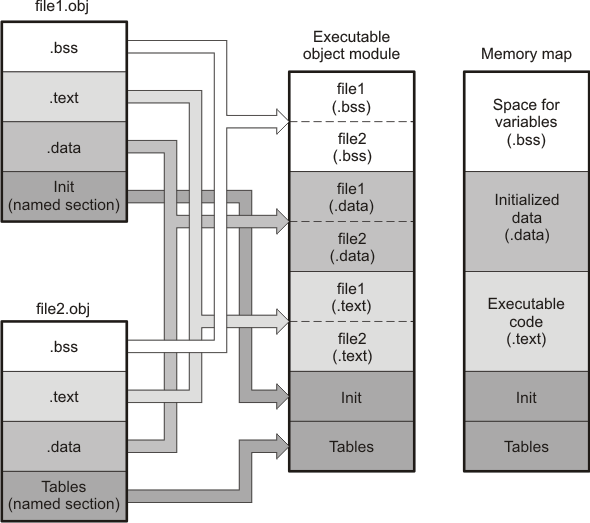
\includegraphics[width=.75\linewidth,keepaspectratio]{art/obj-to-elf-to-mem.png}
	\caption{Combining Input Sections to Form an Executable Object Module.\cite{online:linking}}
	\label{fig:link-mult-files}
\end{figure}

The linker's role in the building process is to combine each of the object files given as input into an executable file, or in the case of this thesis, a dynamic library. \autoref{fig:link-mult-files} better illustrates that concept. At linking time, \texttt{ld} groups the same segments from each \texttt{.o} file together and lays them sequentially in the executable object. Since object files can be given in an arbitrary order, the linker can make no guarantee on the final layout on its own.

In addition, while combining the object files together, the linker also resolves the undefined \textit{external} symbols, variables declared in one object file but used in another. 

Just like source code determines the resulting output of the compiler, it is also possible to control the linking process through the use of a linker script\cite{online:ld-scripts}. Even though, in most cases, users of the GNU linker don't provide a custom script, it is possible to specify one at linking time. 

Using such a script offers much more granularity to the developer in terms of which section gets put where in the executable object. In the field of embedded systems, this is particularly useful. Since components like non-volatile flash memory can be adressable by the CPU\cite{online:flash-ram}, it lets the developer decide whether certain sections should be written to flash (e.g. addressed from 0x10000 to 0x50000) or just be allocated in RAM before running the program.

\begin{listing}[H]
	\vspace{12pt}
	\begin{minted}{c}
SECTIONS
{
	. = 0x10000;
	.text : { *(.text) }//$\label{line:link-ex}$
	. = 0x8000000;
	.data : { *(.data) }
	.bss : { *(.bss) }
}
	\end{minted}
	\caption{Simple example of a GNU \texttt{ld} linker script.}
	\label{code:link-script-ex}
\end{listing}

One can read the example linker script in \autoref{code:link-script-ex}  sequentially. On line \ref{line:link-ex}, the script lays out the \texttt{.text} sections of all the object files sequentially inside the executable object's own \texttt{.text} section. This newly created section starts at address 0x10000 (represented by the "." keyword, the \textit{location counter}\cite{online:gnu-ld}). Then, the linker does the same thing for the \texttt{.data} and \texttt{.bss} sections, starting at address 0x8000000.

\subsection*{Clustering Flight Software Sections}
Since managing memory is always easier when it is contiguous, the first step that was taken to access the flight software memory was to group the sections of the relevant files together. This was done using a custom linker script. To make sure not to leave out any section, the default GNU \texttt{ld} linker script was used to make sure to start from a valid point. This script could be outputted from a shell with 
\begin{minted}{bash}
ld --verbose
\end{minted}
From that point, it was possible to partition the essential sections of the DAS object files only by changing the already valid script. These sections could be clustered in a special section of an intermediate shared object \pathmono{libBbpSim-intermediate.so}. 

As previously stated, one of the linker's job when building an executable is to resolve undefined symbols across all object files and to "interlink" them together. To do that, \texttt{ld} starts by looking in other object files to locate and set the correct addresses. Despite that, if said symbols are not defined in any object files, \textit{they can also be defined in the linker script}. This has two major implications: 
\begin{enumerate}
	\item Bi-directional transmission of values is possible (C code $\Longleftrightarrow$ linker).
	\item The source code can never know in advance the value of the undefined symbol if it's only defined during the linking phase.
\end{enumerate}

By harvesting these concepts together, two new contiguous sections of DAS variables in \pathmono{libBbpSim-intermediate.so} could be constructed. They are shown in \autoref{code:link-script-das}. For both the new \texttt{.das_state_vars_bss} and \texttt{.das_state_vars_data} sections, two symbols were defined as boundary variables to identify the start and end of the section in memory. A pair can be seen at lines \ref{line:bound-start} and \ref{line:bound-end}.

\begin{listing}[htbp]
	\vspace{12pt}
	\begin{minted}{c}
//...
.das_state_vars_data :
{
	__das_state_vars_data_start = .;//$\label{line:bound-start}$
	SORT(*obj/DasSrc/ *.o)(.data .data.* .gnu.linkonce.d.*)
	__das_state_vars_data_end = .;//$\label{line:bound-end}$
}
.das_state_vars_bss (NOLOAD) :
{
	__das_state_vars_bss_start = .;
	SORT(*obj/DasSrc/ *.o)(.bss .bss.* COMMON)
	__das_state_vars_bss_end = .;
}
//...
	\end{minted}
	\caption{Clustering of DAS variables via the \texttt{ld} linker script.}
	\label{code:link-script-das}
\end{listing}

It should also be noted that the \texttt{NOLOAD} parameter of the new \texttt{.das_state_vars_bss} section informed the linker that this memory section was to be zeroed out when the library was loaded, and thus not to allocate this memory inside the shared object itself. Otherwise, the library would be composed of nearly 100MB of zeros. And thanks to the inclusion of section guards, it was now possible to access the start and end addresses of the sections from C using:
\begin{minted}{c}
extern char __das_state_vars_data_start[];
extern char __das_state_vars_data_end[];
\end{minted}

To confirm that the script worked, an output map was produced by \texttt{ld} after the linking process (using \texttt{-Wl,-M=mapfile.map}). An excerpt is given in \autoref{map:ld}. It shows that the sections get created and that the \texttt{.data} and \texttt{.bss} sections of each DAS object file all get correctly mapped in the output file.

\subsection*{Cataloging State Variables}
Once the relevant sections of memory related to DAS were correctly laid out after the linking process, it was now a matter of deducing the address of each of these variables inside the resulting shared object. As the outputted file was in the ELF format, an ELF analyzing tool could then be used to get the list of all the variables contained within the relevant section:
\begin{minted}{bash}
objdump --syms -j .das_state_vars_data libBbpSim-intermediate.so
\end{minted}
Once the output was sanitized with \texttt{awk}, a big text file represented in  \autoref{das-symbol-catalog} was produced. This was called the \textit{symbol catalog}. One can observe various components in this file:
\begin{enumerate}
	\item The first line contains the SHA1 sum of the entire DAS source code repository. This was added to associate the list of variables to an existing source code for compatibility purposes.
	\item Each additional line represents a symbol that is contained in the flight software domain. They are laid out in the \verb|[<address> <size> <name>]| format. The addresses and the sizes are outputted in hexadecimal.
	\item The symbols defined as "guards" (\texttt{__das_state_vars_data_start}) earlier in the linker script were also included in this list. Because they don't represent any value in source code but instead hold an address, their size was zero.
\end{enumerate}

\subsection*{Including the Catalog in the Library}
Being able to generate a symbol catalog was very useful. However, there was a problem: with the way it was constructed, that catalog could never be included in the library. The catalog was generated from a finished shared object, but for it to ever be useful, the catalog needed to be accessible by the library at runtime. This created a chicken and egg problem, where both artifacts were dependent on one another.

The dependence was bypassed by transforming the symbol catalog into an object file and re-linking the library once again, including the new transformed catalog. 

Embedding raw bytes inside an executable file has been done since the early days of computing. For instance, it is possible for a malicious programmer to embed executable code within a self-extracting archive file\cite{online:sfx}. In the case of BBPSim, which was an ELF running on an x86 64-bit machine, it was possible to embed the catalog, as a string, \textit{inside} the library itself by first transforming it into a \texttt{.o} file:
\begin{minted}{bash}
objcopy --input binary --output elf64-x86-64          \
--binary-architecture i386:x86-64                     \
--rename-section .data=.das_state_vars_catalog_string \
das-symbol-catalog.txt                                
\end{minted}

This put the raw bytes of the catalog in the \texttt{.das_state_vars_catalog_string} section of the \pathmono{das-symbol-catalog.o} file.

The second part consisted in correctly laying out those bytes in the second and final shared object, \pathmono{libBbpSim.so}. This was done by once again taking advantage of the linker script in \autoref{code:link-script-das} to add an additional section, \texttt{.das_state_vars_catalog_string}.

Finally, all the object files both from the BBPSim and DAS domains could be linked a second time, together with \pathmono{das-symbol-catalog.o}. The resulting \pathmono{libBbpSim.so} file would be the last and final shared object. This effectively embedded the symbol catalog's raw bytes, encoded in \gls{ASCII} characters. Executable code inside the library could also refer to the stringized symbol catalog via newly created symbols used as guards for the raw bytes. Those symbols being only defined in the second linking process, it was necessary to tag them as having \texttt{weak} linkage for the linker not to complain on the first linker pass:
\begin{minted}{c}
extern char __attribute__((weak)) _binary_das_symbol_catalog_txt_start[];
extern char __attribute__((weak)) _binary_das_symbol_catalog_txt_end[];
\end{minted}

The results can be better shown by using a binary visualization program\cite{online:binvisio}. \autoref{fig:bin-lib-comp} shows a comparison of the \pathmono{libBbpSim-intermediate.so} and \pathmono{libBbpSim.so} shared objects in binary. Bytes with a value in the \gls{ASCII} character range are represented in blue. Both images read left-to-right with address 0x0 on the left. It is possible to see that a new blue section appear in \autoref{fig:bin-lib-final}, thus confirming that the symbol catalog correctly got included in the final version of the BBPSim library.

\begin{figure}[htbp]
	\centering
	\begin{subfigure}{\linewidth}
		\centering
		
\includegraphics[width=\linewidth, keepaspectratio]{art/bin-lib-intermediate.png}
		\caption{Binary visualization of \pathmono{libBbpSim-intermediate.so}}
		\label{fig:bin-lib-intermediate}
	\end{subfigure}
	\vspace{12pt}
	\begin{subfigure}{\linewidth}
		\centering
		\includegraphics[width=\linewidth]{art/bin-lib-final.png}
		\caption{Binary visualization of \pathmono{libBbpSim.so}}
		\label{fig:bin-lib-final}
	\end{subfigure}
	\caption{Comparison of the resulting libraries after the first and second linking process.}
	\label{fig:bin-lib-comp}
\end{figure}

Since there was no modification to the DAS object files between the two linking process, the variable list taken from \pathmono{libBbpSim-intermediate.so} \textit{was guaranteed} to be the same and in the same order as \pathmono{libBbpSim.so}. This embedding of data also did not violate the ELF specification, which is clear about it's requirements:

\begin{shadedquotation}
[...] sections and segments have no specified order. Only the ELF header has a fixed position in the file.\cite{online:elf-spec}
\end{shadedquotation}

\subsection*{Shared Object Considerations}
As stated previously, the delivery method of BBPSim was done through a shared object, or dynamic library. This brought some challenges pertaining to memory validity, since the behavior of those objects is very particular.

When a program links a shared library, it is the job of the \textit{dynamic linker} to load that library in the program's address space at runtime. This special tool performs many things, from load-time relocation to symbol references resolving\cite{online:elf-reloc}, which are all done before the \texttt{main()} of the program is called. In particular, the dynamic linker starts by mapping the different sections of the dynamic library inside the address space of the program. 

\begin{figure}[htbp]
	\centering
	\begin{subfigure}[t]{.58\linewidth}
		\small
		\centering
		\includesvg[width=\linewidth]{svg/ptr-mem-first-run}
		\caption{Contents on the first run.}
		\label{fig:ptr-mem-first-run}
	\end{subfigure}%
	\begin{subfigure}[t]{.38\linewidth}
		\small
		\centering
		\includesvg[width=\linewidth]{svg/ptr-mem-second-run}
		\caption{Contents on the second run}
		\label{fig:ptr-mem-second-run}
	\end{subfigure}
	\caption{Potential displacement of pointed object with ASLR enabled.}
	\label{fig:mem-displacement}
\end{figure}

In Linux, the concept of \gls{ASLR} tells the dynamic linker to randomize the location at which the shared library's sections are loaded with every program run. A problem arose with the use of pointers in flight software: because of ASLR at restore time, pointer variables would become invalid, since what they pointed would not be located at the same address, like in  \autoref{fig:ptr-mem-second-run}. This problem did not have a straightforward solution. For this reason, \gls{SNC} was asked if disabling \gls{ASLR} on their Linux machine would be reasonable, and the request was accepted. This meant that \pathmono{libBbpSim.so} would always be loaded at the same address, hence avoiding this problem. The address was one of the fields in the checkpointing artifact header (see \autoref{tab:header-fields}).

\subsection*{Summary}
This method of indirect access to DAS variables efficiently served its purpose. It defined a way for the BBPSim domain objects to access flight software memory without requiring the modification of software, since everything happened at build time. It deduced the address of the variables rather than depending on an API like \texttt{GetTheVariable()}. This fulfilled the first necessary condition for a stable restore, defined in \autoref{sec:conditions}. One of the big benefits of this approach was that potential addition of new variables to the flight software would be automatically taken in charge, thus the solution was future-proof.

In \autoref{cha:bbpsim-impl}, how the catalog was used by \gls{BBPSim} is further described.
}
\section{FSW Execution Backup and Restore}\label{sec:das-exec-restore}
In \autoref{sec:bbpsim-charact}, the most important characteristics of the BBPSim environment were discussed. In particular, it was seen that the flight software was a multithreaded application running inside the \gls{BBPSim} environment. Because simulations had to run on a Linux machine, the threading API had to be re-implemented by BBPSim to be built on top of the POSIX threads library (\textit{pthread}), which is extensively supported by Linux. 

Saving the execution "point" of each thread was an important part of the design of the checkpointing feature in BBPSim. At restore time, it was vital to put back the threads execution to the point they were before in the code. However, playing with threads was not trivial, since they are an entity that is completely abstracted in C code.

In this section, some approaches that attempted to resolve the execution restore problem are first of all described, along with why they didn't work or couldn't apply in the case of BBPSim. Then, a description of the checkpointing, saving and restoring operations that were adopted in this thesis is given, together with how they fulfill the last two necessary conditions to a stable flight software restore, given in \autoref{sec:conditions}. 

\subsection*{Possible Solutions}
For simplicity reasons, it is often more useful to reduce the complexity of the problem and then scale up the solution to apply it in the real case. For this thesis, the single-threaded restore had to first be solved before attacking the multithreaded aspect. 

While in a simulation, when it is in standby between two step commands, a flight software thread could hold one of three possible states:
\begin{itemize}
	\item \textbf{Fresh}. The thread was created (using the Deos API function \texttt{createThread()}) at the previous step but never actually given CPU time to execute. The thread is pending on a signal (a semaphore).
	\item \textbf{Mature}. The thread has executed for at least one step. This implies that it has called \texttt{waitUntilNextPeriod()} at least once.
	\item \textbf{Dead}. The thread was terminated at the last step, either by itself or another running thread.
\end{itemize}

Three different strategies were attempted to solve the execution restoring problem. One can take \autoref{code:example-task} as an example of a flight task loop to follow through.
\begin{enumerate}
	\item \textbf{Restart back fresh and mature threads from scratch}. This had obvious problems.  Cold-starting all the threads alive when restoring would mean the task preamble (everything \textit{before} the infinite loop) would get executed twice: once at the first simulation and a second time when restoring. Since embedded utilities like mutexes also got restored, the flight software would try to re-create them when restoring. This would inevitably create runtime errors.
	
	\item \textbf{"Replay" the mature threads until their first \texttt{waitUntilNextPeriod()}}. This implied that the \texttt{create*()} Deos API functions had to somehow be skipped, such that no embedded utility was created. The thread would then be replayed until its \texttt{waitUntilNextPeriod()}.
	
	Since \gls{BBPSim} was an \gls{ELF} dynamic library, this option consisted in hooking on these API calls, and redirecting them to stub functions that did nothing. The strategy was possible by using a complex set of operations that overwrote addresses in the look-up table used to resolve dynamic library function addresses, the \texttt{.rel.plt} section.\cite{online:shoumikhin}.
	
	This would have been a good solution, if only for the fact that tasks could contain more than one \texttt{waitUntilNextPeriod()}. There was nothing prohibiting a task to call \texttt{waitUntilNextPeriod()} in its preamble, for example. There was actually many occurrences of this in the flight software, for instance when threads wait for messages from other threads before starting their own task loop.
	
	With this in mind, it was necessary to find out \textit{at which} instance of \texttt{waitUntilNextPeriod()} the thread was saved, and when exactly should the Deos API be "re-enabled". This was considered as a poor approach with too many corner cases to be implemented effectively.
	
	\item \textbf{Reconstruct the entire threads}. This was the candidate kept for this thesis. Choosing this solution implied that everything required to reconstruct the thread needed to be included in the checkpointing artifact, hence the last two necessary conditions of \autoref{sec:conditions}. 
	
	The process relied on two facts: 1. \pathmono{libBbpSim.so} was always loaded at the same address no matter the simulation, and 2. both saved and restored simulations were ran on the same x86-64 machine. 
\end{enumerate}

In the previous sections, it was seen that, to restore back a simulation to its previous state, one had to backup two components pertaining to flight software execution: one set of CPU registers per thread and one execution stack per thread. In the following sections, the strategy used to gather these components is further detailed.

\subsection*{Checkpointing the CPU Register Set}
The first step in saving a thread's execution state was to come up with a way to make the flight software code checkpoint itself. In particular, it was important to obtain a set of registers associated with that thread at the end of every simulation step.

Saving such a register set was absolutely necessary to restore the flight threads without stability issues. The registers contained important information about what the thread was doing. In particular, this set contained the \textit{program counter}, pictured in \autoref{fig:x86-regs}, which itself held the address of the machine instruction the thread would be currently executing. The register set also contained the stack pointer, which pointed on top of the thread's execution stack.

For obvious reasons, it was vital to save this register set \textit{at the right time} in the execution. If the registers were snapshotted at the wrong moment, the program counter would not be pointing to a viable instruction, which would make the restore operation crash. This problem was highlighted by the thread scheduling technique implemented by BBPSim. In \autoref{fig:step-cmd}, it was shown that flight software threads were executed one after another at every simulation step. In practice, this mechanism was implemented with two semaphores. Each thread was pending on a "go" semaphore inside BBPSim's \texttt{waitUntilNextPeriod()} reimplementation. Once the scheduler signaled the semaphore, the thread executed a task loop until it returned inside the \texttt{waitUntilNextPeriod()} function, which signaled back to the scheduler that the thread was done. This procedure is shown in \autoref{code:thr-sched-bbpsim}.

\begin{listing}[htpb]
	\centering
	\begin{minipage}{.5\textwidth}
	\begin{minted}{c}
void Task() {
	//task premable here
	
	while(true) {
		//task loop content here
		waitUntilNextPeriod();
	}
}
	\end{minted}
	\end{minipage}%
	\begin{minipage}{.5\textwidth}
	\begin{minted}{c}
//re-implementation of Deos API
void waitUntilNextPeriod() {
	//loop finished, signal returned
	sem_post(&return_sem);
	//wait for go from scheduler 
	sem_wait(&go_sem);
}
	\end{minted}
	\end{minipage}
	\caption{Thread scheduling procedure in BBPSim.}
	\label{code:thr-sched-bbpsim}
\end{listing}

If the register snapshot happened after a simulation step (using \mintinline{c}|ptrace()| like \gls{CRIU} in \autoref{sec:criu}), all the threads would be waiting inside the \mintinline{c}{sem_wait()} function, which relied on a semaphore artifact that would not be valid anymore at restore time. Therefore, another approach was needed.

The solution chosen for this problem needed the thread to checkpoint \textit{itself}, in order to gather its own set of registers from within its own domain (i.e. inside DAS code). Requirement U02 did however forbade any modification to the flight software. Consequently, the injection of checkpointing code within the flight software was taken as the main strategy. By redefining the \texttt{waitUntilNextPeriod()} symbol, it was possible to inject code that would save the registers at the right moment. This could be done by using the compiler's preprocessor to convert source code before actually compiling the code, like in \autoref{code:chkpt-inject}. By harnessing the GNU C library's types and functions for user-implemented context switching\cite{online:getcontext}, this injection would transform the flight software at compilation to checkpoint itself at the end of every loop, before calling the real \texttt{waitUntilNextPeriod()}. 
\begin{listing}[htpb]
	\centering
	\begin{minted}{c}
#define waitUntilNextPeriod()                         \
do                                                    \
{                                                     \
	ucontext_t* chkpt = GetThreadCheckpointSaveSlot();\
	getcontext(chkpt);                                \
	waitUntilNextPeriodReal();                        \ 
} while(0)

void waitUntilNextPeriodReal() //<- redefined
{
	//semaphore signaling here
}
	\end{minted}
	\caption{Injection of checkpointing code in the flight software.}
	\label{code:chkpt-inject}
\end{listing}

This had big benefits, because register snapshots (done with \mintinline{c}|getcontext()|) would be done inside flight software code, and would thus enable BBPSim to restart back the execution inside the task loop directly. The restored thread would then run until it called \texttt{waitUntilNextPeriodReal()} to wait for the scheduler's "go" signal.

Because the \gls{BBPSim} library would always be loaded at the same address, the program counter that would get saved at this stage would still be valid at restore time. It didn't matter if this was the first simulation or a second restored simulation, the PC would remain valid in-between because it would be pointing to the same instruction. 

This effectively satisfied the second necessary condition for a stable restore, defined in \autoref{sec:conditions}, which was to save the register set of all threads.

\subsection*{Execution Stack Layout}
Properly understanding how the reconstruction of threads was accomplished requires one to first grasp basic execution stack operations principles. As the target machine was based on the x86-64 architecture, this thesis focuses on call stacks produced by this architecture, although the concepts might very well be applicable to others.

The execution stack (also called \textit{call stack}) is a data structure that holds information about the series of functions that were called up to present time. There is one stack per thread of execution in a given program. The stack is a low-level object that keeps track, for every caller function, of the point where the execution should be resumed after the callee returns. This is done through the use of stack frames, which represent calls to subroutines that haven't yet returned. The general layout of this structure in memory is pictured in \autoref{fig:call-stack-layout}, where a caller (\texttt{DrawSquare}) calls a callee (\texttt{DrawLine}). In the x86 architecture, the stack is downward-growing (i.e. from high address to low).

\begin{figure}[htbp]
	\centering
	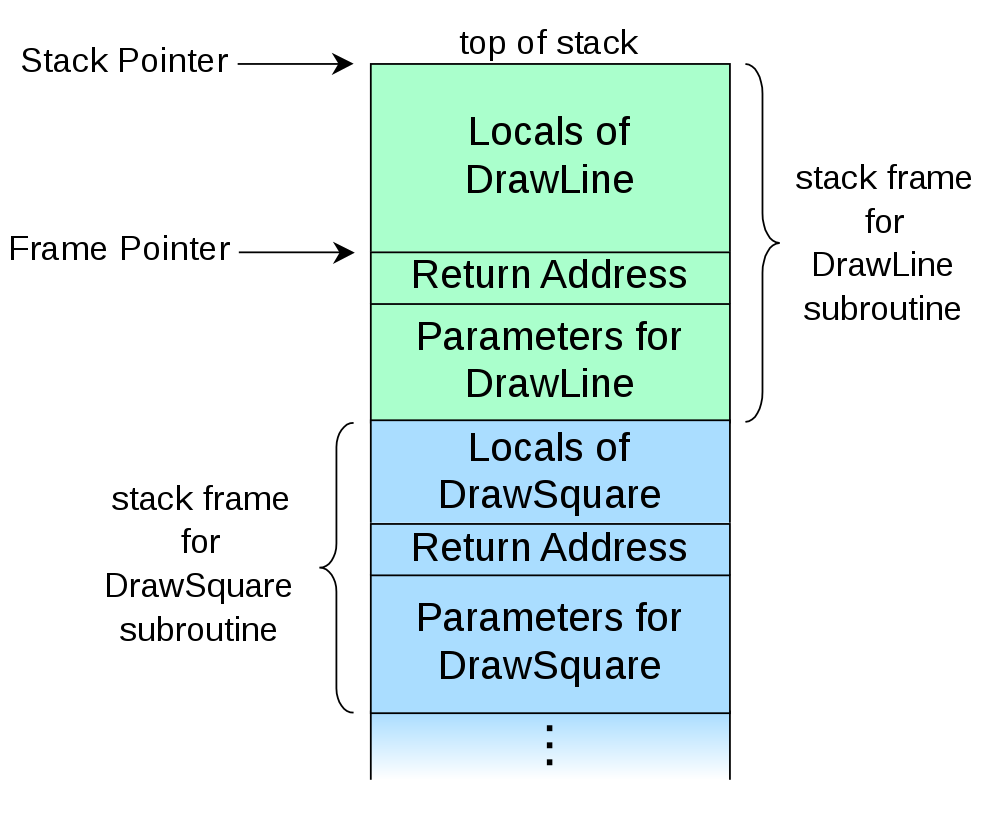
\includegraphics[width=.6\linewidth,keepaspectratio]{art/call-stack-layout.png}
	\caption{Call stack layout for downward-growing stacks\cite{online:stack-img}}
	\label{fig:call-stack-layout}
\end{figure}

The image also shows other important items for proper call stack operations. The \textit{stack pointer} (also in \autoref{fig:x86-regs}) is a CPU register that always points to the top of the stack, at the last accessible address. Another notable CPU register is the \textit{frame pointer}, or base pointer (\texttt{rbp}), which points at the base of the currently active stack frame. 

\subsection*{Accessing Thread Execution Stacks}
When using the usual \mintinline{c}|pthread_create()| API function, one simply has to provide a function as a parameter to create a new thread. Using the default parameters, this call makes the operating system allocate memory for the thread's stack, and then schedules it\cite{online:pthread-create}.

It is however possible for users of the POSIX threads library to specify a region of memory to use as stack space by specifying the attributes with \mintinline{c}|pthread_attr_setstack()|. This simple solution for thread stack execution access by BBPSim was thus chosen. Before starting any flight software thread, \gls{BBPSim} was modified to allocate 2MB of memory for it, which was considered to be sufficient for this application. It should be noted that this block of memory was required to be page-aligned to a virtual memory page. As a result, BBPSim held a reference to every thread's stack. It was then possible to include them in the checkpointing artifact, hence satisfying the third and last necessary condition for a stable restore.

\subsection*{Reconstructing Flight Software Threads}
Once the necessary components were saved as part of the first BBPSim simulation, both the fresh and mature threads had to be brought back in the same state as they were before. Nevertheless, the past execution stacks and register sets weren't enough, by themselves, to be able to restart the past threads. Some meticulous manipulations of that data had first to be done. 

Indeed, the reconstruction of flight software threads had to reconcile two different ecosystem together. From the operating system's point of view, the threads that were spawned in the second simulation run were completely different from those on the first. But from the flight software's perspective, the threads had to be, functionally speaking, the same. In that sense, one couldn't simply copy the old stack onto the new and expect the thread's execution to continue seamlessly. One reason for this is that important scheduling information was contained at the base of the stack, at higher addresses. 

To solve the problem, this thesis presents a way to reconstruct the old flight software threads by using new threads and meticulously replacing their stack frames with old frames. 

First of all, it was important to define the concept of \textit{user stack}. The stack of a pthread was divided in four main spaces, like \autoref{fig:stack-spaces} shows. The first two spaces were defined as containing all call frames pertaining to functions in the C and pthread libraries respectively, which use low-level Linux routines to coordinate the creation of the thread. As for the user stack space, it was defined as being the portion that contains all the frames related to \textit{user-defined functions}. In that sense, the \textit{user stack start} was defined as being located at the first 64-bit-aligned address after the pthread stack space. 
\begin{figure}[htbp]
	\centering 
	\includesvg[width=.8\textwidth]{svg/stack-spaces}
	\caption{Division of the execution stack into spaces.}
	\label{fig:stack-spaces}
\end{figure}

Because C code abstracts low-level constructs, finding the beginning of the user stack required the use of assembly. This was done by using \gls{GCC}'s inline assembly tools at the beginning of the first user function (the one provided to \mintinline{c}|pthread_create()|), as \autoref{code:usr-stk-start} shows\cite{online:inline-asm}. Once this address could be accessed, it was possible to deduce the total user stack start offset in any stack $s$ by subtracting the stack top's address:
\[
	\Delta_{usr}=s_{usr}-s_{top}
\]
Once this offset was obtained, it was crucial to include it in the checkpointing artifact, since pthreads don't necessarily \textit{always} have the same $\Delta_{usr}$. 
\begin{listing}[htpb]
	\centering
	\begin{minted}{c}
void bbpsimThreadEntry() {
	uint64_t x[4]; //0x20 bytes 
	asm volatile("mov %%rsp, %0  \n\t" //get current stack pointer
                 "addq $0x20, %0 \n\t" 
                 : "=r" (fswthread->m_pi8StartUserStack) //=$s_{usr}$
                 :);
	flightSoftwareTask(); //<- call never returns
}
	\end{minted}
	\caption{Capture of the user stack start.}
	\label{code:usr-stk-start}
\end{listing}

From then, it was possible to reconstruct the thread's execution stack the way it was before by copying only the user and unused portions of the old stack onto the new. This operation was done by the thread itself, using another inline assembly routine located in the restoring function. This stack-copying operation had to be done meticulously. It was important not to "pollute" the resulting stack, and thus this is why assembly was once again the perfect candidate. The ability to handle the registers manually could provide the required granular control. The complete thread reconstruction routine is included in \autoref{code:stk-copy-asm}. In the code, it is possible to observe many things. First, the \texttt{copyquadword} subroutine (at line \ref{code:copyqword-beg}) is called many times in order to copy the old user stack on the new one, starting from the correct offset. Then the routine jumps to \texttt{setcontext()}, which overwrites the current register set with the old one. This call should never return, because it sets the program counter to point back into the flight software code. Because \texttt{setcontext()} itself makes use of the stack\cite{online:setcontext}, it was important to first make the stack pointer point at an appropriate address, so as to not pollute the stack portions that were just written to. In the end, making a live thread replace its own stack frames could qualify as a careful stack corruption exercise, which is pictured in \autoref{fig:stack-reconstruction}.

\begin{figure}[htbp]
	\centering
	\begin{subfigure}{.33\linewidth}
		\centering\small
		\includesvg[height=\linewidth]{svg/stack-reconstruction1}
		\caption{Restored thread before}
	\end{subfigure}%
	\begin{subfigure}{.33\linewidth}
		\centering\small
		\includesvg[height=\linewidth]{svg/stack-reconstruction2}
		\caption{Old frames overwritten}
	\end{subfigure}%
	\begin{subfigure}{.33\linewidth}
		\centering\small
		\includesvg[height=\linewidth]{svg/stack-reconstruction3}
		\caption{Copy of the old frames}
	\end{subfigure}
	\caption{Stack reconstruction process.}
	\label{fig:stack-reconstruction}
\end{figure}

Keeping in mind that the \gls{BBPSim} library was always loaded at the same address, replacing the entirety of the new user stack by the old one had big benefits:
\begin{itemize}
	\item \textbf{Backtrace information was preserved}. This meant that, when using GDB to debug a restored simulation, the debugger would correctly find the return addresses in each stack frame (see \autoref{fig:call-stack-layout}) and could thus display the exact call stack that was just restored. The approach "fooled" GDB into thinking this new stack was there all along.
	\item \textbf{Stack variables were preserved}. With the way everything was copied over, even variables allocated on the stack would hold the same value. This meant that function-scoped variables could hold the same value as before.
\end{itemize}

Using this low-level approach, the restoring of a thread was near instantaneous, fulfilling customer requirement DCMS-BBP-56. The only cost was the stack-copying subroutine, which couldn't really be more optimized than the one in \autoref{code:stk-copy-asm}.

\subsection*{Solution Limitations}
Of course, using such a technique brought its lot of drawbacks. Since the old stack was copied integrally, this meant that stack-allocated pointers were put back as well, and thus held the same value as during the first simulation. In flight software, this was mitigated mainly for three reasons: 
\begin{enumerate}
	\item The address of static DAS variables was always the same, so those pointers would point to a valid address.
	\item Dynamic memory allocation wasn't used, so addresses were deterministic. BBPSim objects, though, were allocated dynamically, and some BBPSim-defined Deos types had to be modified to address the issue. This subject is treated in \autoref{cha:bbpsim-impl}. 
	\item The amount of old stack frames to copy back was low. This is because end-of-task-loop calls to \texttt{waitUntilNextPeriod()}, which checkpointed the flight software, were nearly always located in the task loop (i.e. when in the first user stack frame). This characteristic mitigated problems related to using the address of a function-local variable as a pointer parameter to another function, which would have been invalidated by the restoring process. 
\end{enumerate}

This process was also limited in the fact that the \texttt{-fomit-frame-pointer} GCC option unconditionally needed to be enabled. As the x86 architecture states, the frame pointer of the caller is usually pushed on the stack when calling a function\cite{online:x86-abi}. This means that the stack usually contains data that points inside \textit{itself}. As thread stacks were dynamically allocated, and thus were never located at the same place in memory, frame pointers were a big problem. Adding the GCC option when compiling every C and \Cpp file completely removed that limitation by taking out the reliance on the frame pointer entirely. It results in slight modifications to the compiled program, which changes the access to stack-allocated variables to be based on an offset from the \textit{stack pointer} rather than the frame pointer\cite{online:omit-frame-pointer}.

Finally, this solution was definitely not portable. Although this wasn't a problem for BBPSim, using the presented technique to cover a wide range of architecture in a general program would not work without extensively rethinking it. In addition, the use of inline assembly is compiler-specific. Even though GCC is very popular, this stack-copying approach is still locked to this compiler. 



}